\chapter{System Methodology}

This chapter presents the methodology adopted for the development of the proposed Edge-AI-based semiconductor defect classification system. The objective of the system is to accurately classify semiconductor defects while satisfying practical deployment constraints such as low latency, reduced memory usage, and computational efficiency on resource-constrained edge devices.

The overall methodology consists of dataset preparation, image pre-processing, data augmentation, lightweight model selection, transfer learning-based training, performance evaluation, model optimization, and deployment feasibility analysis on edge platforms. In addition, explainability and responsible AI assessment techniques are incorporated to ensure reliable and trustworthy model predictions.

The complete workflow of the proposed system is illustrated in Figure 3.1.

\section{Data collection and Preparation}

The performance of any deep learning–based defect classification system is highly dependent on the quality, diversity, and representativeness of the training dataset. In semiconductor manufacturing, obtaining large-scale labeled defect datasets is a major challenge due to intellectual property restrictions, confidentiality agreements, limited public release of fab inspection data, and the high cost of expert annotation. As a result, publicly available semiconductor image datasets often contain limited defect categories, low sample counts, or incomplete metadata.

To address these practical constraints, a hybrid dataset generation strategy was adopted in this work by combining publicly available semiconductor defect images with synthetically generated defect samples. This approach enabled the creation of a balanced and sufficiently diverse dataset suitable for training and evaluating lightweight deep learning models under realistic research constraints.

\subsection{Data Collection Approach}
Since access to proprietary industrial semiconductor datasets was not available, the dataset used in this research was developed from two complementary sources:

\subsubsection{Public Semiconductor Defect Datasets}
Publicly available semiconductor inspection datasets were explored to obtain real defect image samples representing defects observed during wafer or die inspection. These datasets provided realistic defect textures, process noise characteristics, and manufacturing variations that are difficult to manually reproduce.
Public datasets were used primarily to capture:
\begin{itemize}
\item Real inspection image characteristics
\item Practical background noise
\item Irregular defect boundaries
\item Real-world imaging conditions
\item Variations in illumination and contrast
\end{itemize}

\subsubsection{Synthetic Defect Image Generation}
Due to the limited number of publicly available labeled samples for certain defect classes, synthetic images were generated to supplement the dataset. Artificial defect patterns were created using geometric structures, shape distortions, line interruptions, cracks, and conductive path abnormalities resembling semiconductor layout defects.
Synthetic data generation helped overcome:
\begin{itemize}
    \item Small sample size
    \item Missing defect classes
    \item Severe class imbalance
    \item Limited diversity in pattern orientation and scale
\end{itemize}

\subsection{Defect Classes Considered}
The proposed dataset was constructed using five representative semiconductor defect classes relevant to lithography, interconnect, and layout inspection tasks.

\subsubsection{LER (Line Edge Roughness)}
LER refers to irregular or rough edges along patterned semiconductor lines caused by lithography or etching process variations. Excessive edge roughness may degrade device performance and dimensional accuracy.

\subsubsection{Crack}
Crack defects represent visible fractures or discontinuities in material layers, lines, or structural regions. These defects can reduce reliability and may lead to open circuit failure.

\subsubsection{Malformed Via}
Malformed via defects occur when inter-layer connection holes are incorrectly shaped, partially formed, shifted, or deformed. Such defects can affect electrical connectivity between layers.

\subsubsection{Open}
Open defects represent broken conductive paths where current flow is interrupted due to missing metal connection or structural discontinuity.

\subsubsection{Short}
Short defects occur when two conductive regions become unintentionally connected, resulting in undesired electrical conduction.

These five classes were selected because they cover both geometric and electrical failure modes commonly studied in semiconductor inspection systems.

\begin{figure}[h]
    \centering
    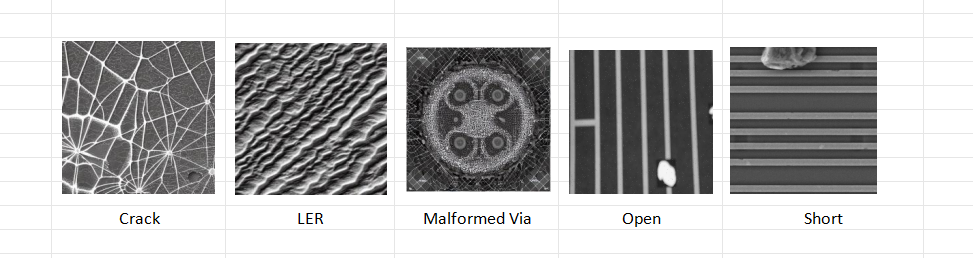
\includegraphics[width=0.8\textwidth]{Intro_Defect_types.png}
    \caption{Defect types}
    \label{fig:gradcam}
\end{figure}

\subsection{Data Challenges}
During dataset preparation, several practical challenges were identified.
\subsubsection{Class Imbalance}

Some defect categories had fewer available samples than others. For example, crack and malformed via images were less common than open or short patterns. Such imbalance may bias the model toward majority classes.

\subsubsection{Limited Access to Real Industrial Data}

Semiconductor manufacturers typically restrict access to defect images because they may reveal proprietary layouts, process technologies, yield issues, or customer-sensitive information. Therefore, large industrial datasets were not accessible.

\subsubsection {Variability in Defect Appearance}

Defects may vary significantly in:
\begin{itemize}
\item Shape
\item Orientation
\item Size
\item Intensity
\item Contrast
\item Position
\item Background texture
\end{itemize}
This increases classification difficulty and requires robust preprocessing and augmentation techniques.

\subsection{Data Pre-processing}
Before model training, all collected images were preprocessed into a consistent format suitable for convolutional neural networks.

\subsubsection {Image Resizing}

Images originally collected from different sources contained varying resolutions. To maintain compatibility with pretrained lightweight CNN architectures, all images were resized to:

224 × 224 pixels

This size was selected because it is the standard input dimension for many ImageNet-pretrained models such as MobileNet, ResNet, and EfficientNet.

Benefits include:
\begin{itemize}
\item Uniform tensor dimensions
\item Faster batch processing
\item Lower memory usage
\item Compatibility with transfer learning models
\end{itemize}

\subsubsection {Normalization}

Pixel intensity values were normalized using standard ImageNet mean and standard deviation values:
\begin{itemize}
\item Mean = [0.485, 0.456, 0.406]
\item Std = [0.229, 0.224, 0.225]
\end{itemize}
Normalization improves numerical stability and accelerates convergence during training. It is especially useful when using transfer learning from ImageNet-pretrained networks.

\subsection{Data Augmentation}

To improve generalization and reduce overfitting, data augmentation techniques were applied during training. Augmentation artificially increases dataset diversity by generating transformed versions of existing images while preserving defect identity.

The following transformations were used:

 \subsubsection{Rotation}

Images were randomly rotated within a specified angle range. This helps the model learn rotational invariance since defects may appear at different orientations.

 \subsubsection{Flipping}

Horizontal and vertical flipping were used where physically meaningful. This improves robustness to mirrored pattern appearances.

 \subsubsection{Scaling / Zooming}

Random scaling allowed the model to recognize defects appearing at different sizes or magnification levels.

\subsubsection{Benefits of Augmentation}
\begin{itemize}
\item Improved model generalization
\item Reduced overfitting
\item Better minority class learning
\item Increased robustness to real inspection variability
\end{itemize}

\subsection{Dataset Split}

The complete dataset was divided into three mutually exclusive subsets for unbiased training and evaluation.

\subsubsection {Training Set}

Used to train the deep learning model and update network weights.

\subsubsection{Validation Set}

Used during training to tune hyperparameters, monitor overfitting, and select the best-performing model checkpoint.

\subsubsection {Test Set}

Used only after training completion to measure final generalization performance on unseen data.

\begin{figure}[htbp]
\centering

\begin{minipage}{0.48\textwidth}
    \centering
    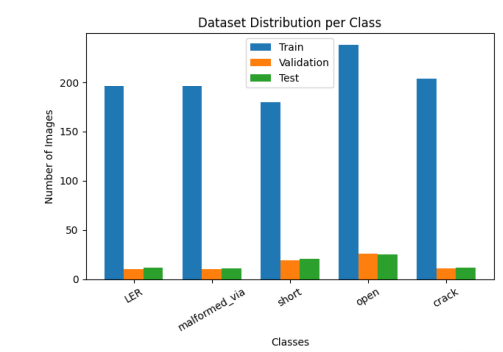
\includegraphics[width=\linewidth]{Dataset_Distribution.png}
    \caption*{(a) Chart of Dataset distribution}
\end{minipage}
\hfill
\begin{minipage}{0.48\textwidth}
    \centering
    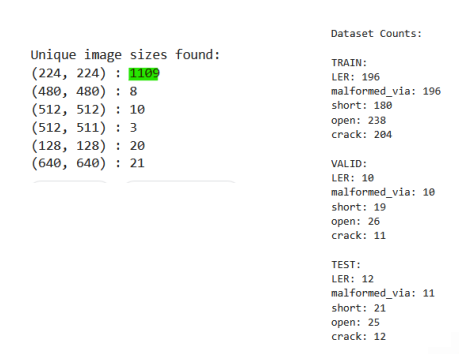
\includegraphics[width=\linewidth]{Dataset_Stat.png}
    \caption*{(b) Dataset Statistics}
\end{minipage}

\caption{Performance comparison using bar chart and statistical summary}
\label{fig:bar_stats}
\end{figure}
A typical split ratio used in this work was:

Training Set: 90%
Validation Set: 05%
Test Set: 05%

\subsection{Summary}
Due to the limited availability of real industrial semiconductor defect datasets, a hybrid dataset strategy combining public and synthetic samples was adopted. Five important defect classes were considered. Pre-processing, normalization, augmentation, and systematic train-validation-test splitting were performed to ensure robust model training and reliable evaluation of the proposed Edge-AI framework.

\section{Model Architecture and Training Methodology}

\begin{figure}[H]
    \centering
    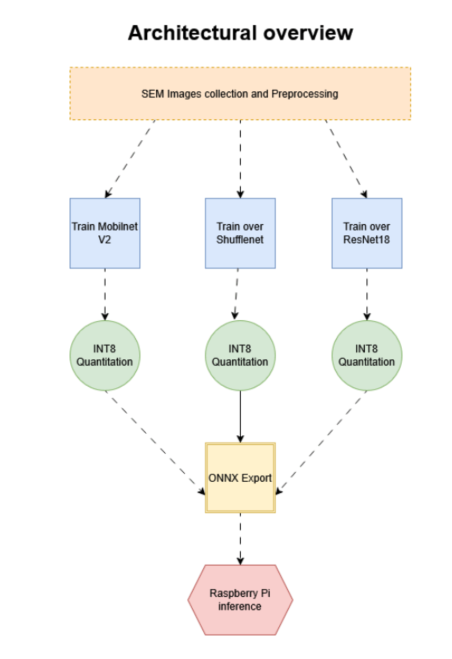
\includegraphics[width=0.4\textwidth]{Architecture_Overview.png}
    \caption{Architectural Overview}
    \label{fig:Architectural Overview}
\end{figure}

\begin{figure}[H]
    \centering
    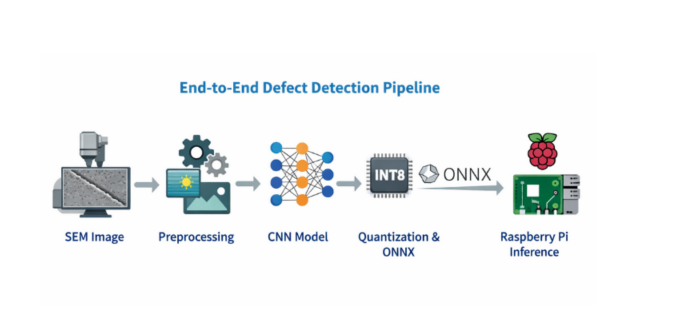
\includegraphics[width=0.8\textwidth]{End_to_End_Pipeline.png}
    \caption{End to End Pipeline}
    \label{fig:End to End Pipeline}
\end{figure}

Selecting an appropriate deep learning architecture is a critical step in the development of an Edge-AI–based semiconductor defect classification system. In practical deployment environments, the model must not only achieve high classification accuracy but also satisfy hardware constraints such as low memory usage, reduced computational complexity, and fast inference speed.

Therefore, this work focuses on lightweight and edge-deployable convolutional neural network (CNN) architectures that are suitable for deployment on embedded platforms such as Raspberry Pi and similar low-power devices. To establish a balanced comparison, three architectures were selected: MobileNetV2, ShuffleNet, and ResNet18.

These models represent different design philosophies:
\begin{itemize}
 \item MobileNetV2 – optimized for mobile and embedded devices using depthwise separable convolution
 \item ShuffleNet – highly efficient architecture designed for low-compute hardware
 \item ResNet18 – compact residual network used as a strong baseline model
\end{itemize}
Each model was trained and evaluated on the prepared semiconductor defect dataset under identical experimental conditions.

\subsection{Edge Deployable Model Selection Criteria}
The selected models were chosen based on the following criteria:

\subsubsection{Low Parameter Count}

Smaller models require less storage and memory, making them suitable for embedded systems.

\subsubsection{Reduced Computational Cost}

Lower FLOPs (floating point operations) enable faster inference.

\subsubsection{Transfer Learning Availability}

Pretrained ImageNet weights help improve performance with limited semiconductor datasets.

\subsubsection{Real-Time Inference Capability}

Models should support low-latency classification for inline semiconductor inspection systems.

\subsection{Model 1: MobileNetV2}
Architecture Overview

MobileNetV2 is a lightweight convolutional neural network specifically designed for mobile and edge devices. It introduces:
\begin{itemize}
   \item Depthwise Separable Convolution
   \item Inverted Residual Blocks
   \item Linear Bottleneck Layers
\end{itemize}
These innovations significantly reduce computation while preserving accuracy.

\subsubsection{Why MobilnetV2 is selected}
MobileNetV2 is highly suitable for semiconductor edge inspection because it offers:
\begin{itemize}
\item Low memory footprint
\item Fast inference speed
\item Strong classification performance
\item Efficient deployment on Raspberry Pi
\end{itemize}

\subsubsection{ Training Methodology}

The pretrained ImageNet MobileNetV2 model was used as the base network. The final fully connected classification layer was replaced with a custom layer containing five output neurons corresponding to: LER, Crack, Malformed Via, open and short
\subsubsection{ Fine-Tuning Strategy}
\begin{itemize}

\item Early layers frozen initially
\item Final layers retrained on semiconductor dataset
\item Later partial fine-tuning applied
\end{itemize}

\subsection{Model 2: ShuffleNet }

\subsubsection{Architecture Overview}
ShuffleNet is an ultra-lightweight CNN architecture developed for extremely resource-constrained devices. It uses:
\begin{itemize}
\item Pointwise Group Convolution
\item Channel Shuffle Operation
\item Efficient feature reuse
\end{itemize}

These techniques reduce complexity while maintaining useful feature extraction capability.

\subsection{Why Shufflenet is selected}

ShuffleNet is ideal for edge benchmarking because:
\begin{itemize}
\item Very low parameter count
\item Fast CPU inference
\item Suitable for real-time embedded systems
\end{itemize}

\subsubsection{Training Methodology}

The pretrained ShuffleNet model was initialized using ImageNet weights. The original classifier was replaced with a five-class output layer.

\subsubsection{Fine-Tuning Approach:}
\begin{itemize}
\item Base layers retained pretrained weights
\item Final classifier retrained
\item Entire network fine-tuned with low learning rate
\end{itemize}

\subsection{Model 3:ResNet18 }
\subsubsection{Architecture Overview}

ResNet18 is a residual convolutional neural network containing 18 layers. It uses skip connections that help train deeper networks by avoiding vanishing gradients.

\subsection{Why ResNet18 is selected}

Although larger than MobileNetV2 and ShuffleNet, ResNet18 provides:
\begin{itemize}
\item Strong feature extraction capability
\item Stable convergence
\item Reliable benchmark baseline
\end{itemize}
It serves as a reference model to compare accuracy versus efficiency trade-offs.

\subsubsection{Training Methodology}

A pretrained ResNet18 model was used. The final fully connected layer was replaced with a five-class classifier.

\subsubsection{Fine-Tuning Strategy}
\begin{itemize}
\item Entire network fine-tuned after classifier replacement
\item Lower learning rate used for stable convergence
\end{itemize}

\section{Model Architecture and Training Methodology}
Deep learning models trained in research environments are usually developed on high-performance systems equipped with GPUs, large memory, and powerful processors. However, in practical semiconductor manufacturing environments, deploying these models directly on edge hardware such as Raspberry Pi, industrial embedded controllers, or low-power CPUs presents several challenges.

Edge devices operate under limited computational resources, restricted memory, lower power budgets, and real-time response requirements. Therefore, a trained model must be optimized before deployment so that it can perform efficient inference without significantly compromising classification accuracy.

This section explains the need for edge optimization techniques such as quantization and the importance of ONNX as a deployment framework.

\subsection{Why Edge Optimization is Required}
Although a model may perform well during training, direct deployment of an unoptimized model on edge hardware can lead to:
\begin{itemize}
    \item Slow inference speed
    \item High memory usage
    \item Long startup/loading time (long bootup)
    \item Excessive CPU utilization
    \item Thermal throttling
    \item Increased power consumption
    \item Poor real-time usability
\end{itemize}
In semiconductor production lines, such delays can interrupt inspection flow and reduce throughput. Therefore, optimization is essential.

\subsection{Quantization}
Quantization is the process of reducing numerical precision of model weights and activations. Usually it reduces model size and computational cost.

\subsubsection{Importance of quantization in our use case}
\begin{itemize}
    \item Faster Inference: nteger or lower-precision arithmetic is faster on many CPUs.
    \item Lower Memory Usage: Smaller weights occpy less RAM
    \item Reduced Storage Size: Compressed models are easier to deploy and transfer.
\end{itemize}

Devices such as Raspberry Pi have limited RAM and CPU capability. Quantization helps run models more efficiently without needing expensive GPU hardware.

\subsection{Why ONNX is Needed}
ONNX (Open Neural Network Exchange) is a standard format for representing machine learning models independent of the original training framework.

It allows a model trained in PyTorch or TensorFlow to be exported into a portable optimized format.

\subsubsection{Problems with Direct Framework Deployment}
Deploying PyTorch/TensorFlow models directly on edge devices may require:
\begin{itemize}
\item Large software installations
\item Extra runtime dependencies
\item Higher memory overhead
\item Slower CPU inference
\item More complex deployment setup
\end{itemize}
This is inefficient for embedded systems.

\subsection{Quantization + ONNX Together}
A strong deployment pipeline can be formed as:

Train Model → Convert to ONNX → Apply Quantization → Run on Edge Device

This provides:
\begin{itemize}
\item Smaller model
\item Faster inference
\item Lower RAM use
\item Practical real-time deployment
\end{itemize}

\subsubsection{Summary}
Edge optimization is essential because models trained in high-performance environments are often too heavy for direct embedded deployment. Techniques such as quantization reduce model size, memory usage, and inference latency. ONNX further improves portability and execution efficiency by providing a lightweight standardized deployment format. Together, these techniques make real-time semiconductor defect classification feasible on practical edge devices.


\section{Grad-CAM Usage in the Proposed Semiconductor Defect Classification System}
In this project, Grad-CAM was primarily used as a post-training validation and interpretability tool to examine how the trained deep learning models arrived at their classification decisions. Since the proposed system is intended for semiconductor defect inspection, it is important to ensure that the model predicts a defect class based on the actual defect region rather than irrelevant image patterns.

Therefore, Grad-CAM was integrated into the evaluation stage of the project and applied after model training and testing.

\subsection{How Grad-CAM Was Used in This Project}
After the models (MobileNetV2, ShuffleNet, and ResNet18) were trained on the semiconductor defect dataset, Grad-CAM was generated for test images.
For each input image:
\begin{itemize}
\item The trained model first predicted the defect class.
\item Grad-CAM was then applied to the last convolutional layer of the same model.
\item A heatmap was produced showing the image regions that most influenced the prediction.
\item The heatmap was overlaid on the original semiconductor image.
\item The highlighted region was visually compared with the actual defect location.
\end{itemize}
This process was repeated across multiple correctly classified and misclassified samples.

The main use of Grad-CAM in this work was to validate whether the trained models learned meaningful semiconductor defect features.

\subsection{How It Was Used for Each Defect Class}
Grad-CAM was specifically used to inspect model attention for all five defect categories.

\subsubsection{ LER (Line Edge Roughness)}

Used to verify whether the model focused on irregular line boundaries.

\subsubsection{Crack}

Used to confirm attention on visible fracture regions.

\subsubsection{Malformed Via}

Used to inspect whether the model localized deformed via/contact structures.

\subsubsection{Open}

Used to verify focus on broken conductive paths or missing links.

\subsubsection{Short}

Used to confirm attention on bridging or unintended connected regions.

\subsection{How Grad-CAM Was Used in This Project}
For wrongly predicted samples, Grad-CAM was used to understand the reason for failure.

It helped identify whether the model:
\begin{itemize}
\item Focused on wrong region
\item Ignored subtle defect area
\item Confused visually similar defects
\item Reacted to noise or artifacts
\end{itemize}
This was useful for future improvement through better augmentation, more data, or architecture refinement.

In this project, Grad-CAM was actively used after training as a practical evaluation tool for verifying model behavior. It was used to inspect class-wise attention, compare different architectures, analyze errors, and support final model selection for edge deployment. This ensured that the proposed semiconductor defect classifier made decisions based on real defect regions rather than irrelevant image content, thereby improving reliability for industrial use.